\documentclass{beamer} 
\usepackage{caption}
 \captionsetup{font=scriptsize}
\usepackage{algorithm}
\usepackage{colortbl}% http://ctan.org/pkg/colortbl
\usepackage{booktabs}
\usepackage{adjustbox}
\usepackage[noend]{algorithmic}
\usepackage{fancybox}
\floatname{algorithm}{Procedure}
\renewcommand{\algorithmicrequire}{\textbf{Input:}}
\renewcommand{\algorithmicensure}{\textbf{Output:}}
\usepackage{wrapfig}
\setbeamertemplate{navigation symbols}{}
\setbeamertemplate{footline}[frame number]

\usetheme[height=0mm]{Rochester}

%\setbeamertemplate{footline}%{miniframes theme}
% {%
%   \begin{beamercolorbox}[ht=2.5ex,dp=1.125ex,%
%     leftskip=.3cm,rightskip=.3cm plus1fil]{title in head/foot}%
%     {\usebeamerfont{title in head/foot}\insertshorttitle} \hfill     \insertframenumber%
%   \end{beamercolorbox}%
% }











\colorlet{tableheadcolor}{gray!25} % Table header colour = 25% gray
\newcommand{\headcol}{\rowcolor{tableheadcolor}} %
\colorlet{tablerowcolor}{gray!10} % Table row separator colour = 10% gray
\newcommand{\rowcol}{\rowcolor{tablerowcolor}} %
    % Command \topline consists of a (slightly modified) \toprule followed by a \heavyrule rule of colour tableheadcolor (hence, 2 separate rules)
\newcommand{\topline}{\arrayrulecolor{black}\specialrule{0.1em}{\abovetopsep}{0pt}%
            \arrayrulecolor{tableheadcolor}\specialrule{\belowrulesep}{0pt}{0pt}%
            \arrayrulecolor{black}}
    % Command \midline consists of 3 rules (top colour tableheadcolor, middle colour black, bottom colour white)
\newcommand{\midline}{\arrayrulecolor{tableheadcolor}\specialrule{\aboverulesep}{0pt}{0pt}%
            \arrayrulecolor{black}\specialrule{\lightrulewidth}{0pt}{0pt}%
            \arrayrulecolor{white}\specialrule{\belowrulesep}{0pt}{0pt}%
            \arrayrulecolor{black}}
    % Command \rowmidlinecw consists of 3 rules (top colour tablerowcolor, middle colour black, bottom colour white)
\newcommand{\rowmidlinecw}{\arrayrulecolor{tablerowcolor}\specialrule{\aboverulesep}{0pt}{0pt}%
            \arrayrulecolor{black}\specialrule{\lightrulewidth}{0pt}{0pt}%
            \arrayrulecolor{white}\specialrule{\belowrulesep}{0pt}{0pt}%
            \arrayrulecolor{black}}
    % Command \rowmidlinewc consists of 3 rules (top colour white, middle colour black, bottom colour tablerowcolor)
\newcommand{\rowmidlinewc}{\arrayrulecolor{white}\specialrule{\aboverulesep}{0pt}{0pt}%
            \arrayrulecolor{black}\specialrule{\lightrulewidth}{0pt}{0pt}%
            \arrayrulecolor{tablerowcolor}\specialrule{\belowrulesep}{0pt}{0pt}%
            \arrayrulecolor{black}}
    % Command \rowmidlinew consists of 1 white rule
\newcommand{\rowmidlinew}{\arrayrulecolor{white}\specialrule{\aboverulesep}{0pt}{0pt}%
            \arrayrulecolor{black}}
    % Command \rowmidlinec consists of 1 tablerowcolor rule
\newcommand{\rowmidlinec}{\arrayrulecolor{tablerowcolor}\specialrule{\aboverulesep}{0pt}{0pt}%
            \arrayrulecolor{black}}
    % Command \bottomline consists of 2 rules (top colour
\newcommand{\bottomline}{\arrayrulecolor{white}\specialrule{\aboverulesep}{0pt}{0pt}%
            \arrayrulecolor{black}\specialrule{\heavyrulewidth}{0pt}{\belowbottomsep}}%
\newcommand{\bottomlinec}{\arrayrulecolor{tablerowcolor}\specialrule{\aboverulesep}{0pt}{0pt}%
            \arrayrulecolor{black}\specialrule{\heavyrulewidth}{0pt}{\belowbottomsep}}%









\useinnertheme{rectangles}
\newcommand{\LINEIF}[2]{%
    \STATE\algorithmicif\ {#1}\ \algorithmicthen\ {#2} \ %algorithmicend\ \algorithmicif%
}

\title[Master thesis presentation: Mining adverse events from healthcare data]
{Master thesis presentation: Mining adverse events from healthcare data}
\author[Dries Van Daele]{Dries Van Daele}
\institute{KU Leuven, DTAI}
\date{6 september, 2013}

\begin{document}

\begin{frame}{}
  \titlepage
\end{frame}

\begin{frame}{Problem description}
Problem: voluntary reporting records a fraction of the adverse events\vspace{3 mm}


manual detection
\begin{itemize}
\item is costly
\item is limited in scope
\item is driven by intuition
\end{itemize}
data mining
\begin{itemize}
\item treats all patient data uniformly
\item can reason over all relevant data
\item enables automation
\item makes biases explicit
\end{itemize}
\end{frame}


\begin{frame}{Problem description}
Task: Apply data mining on a given database to perform the detection of adverse events
\begin{figure}
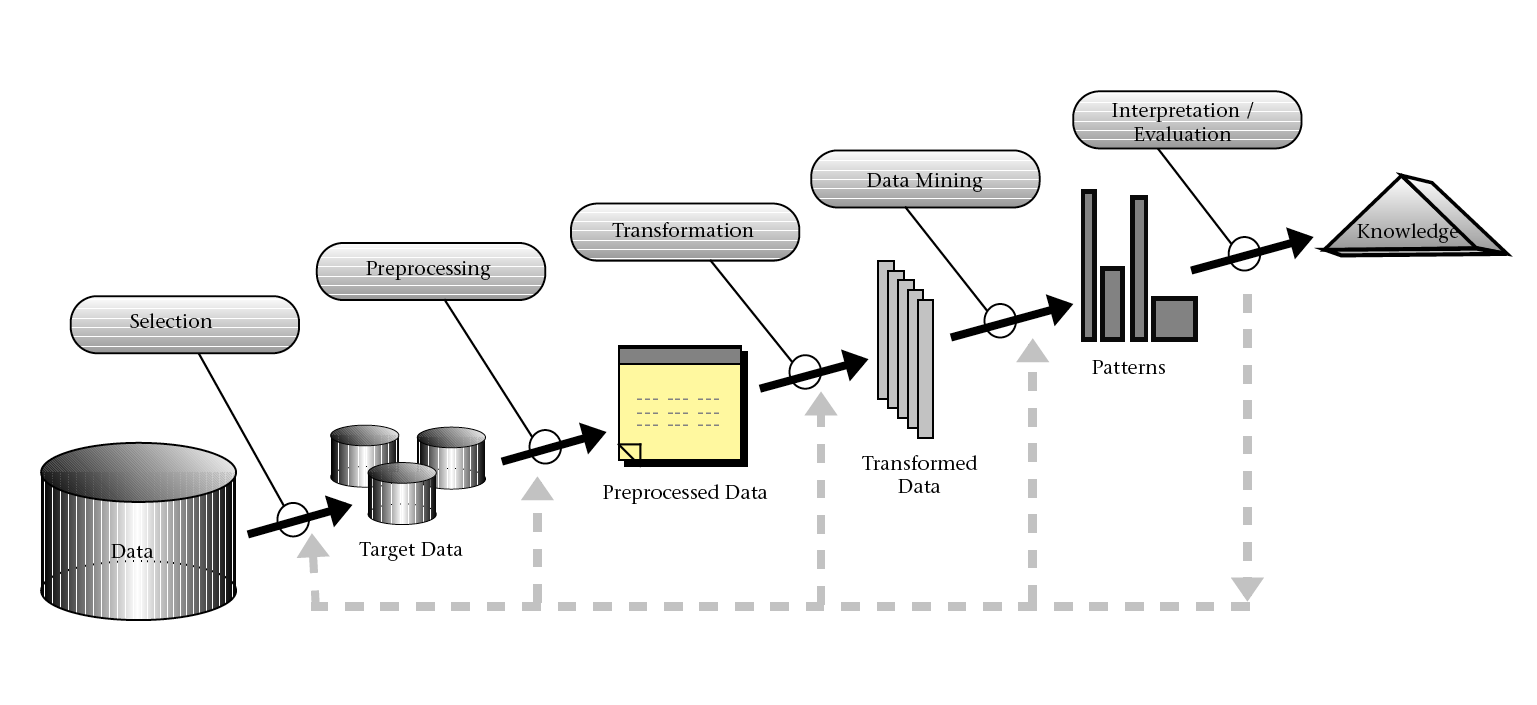
\includegraphics[width=\textwidth,height=.88\textheight,keepaspectratio]{kdd}
{\footnotesize \caption{http://www.kdnuggets.com/gpspubs/aimag-kdd-overview-1996-Fayyad.pdf}}
\end{figure}

\end{frame}


% \begin{frame}{Methodology}
%   \centering
%   % \adjustbox{max height=\dimexpr\textheight/3\relax,
%   % max width=\textwidth}{
%   \begin{tabular}{| l | l | l | l |}
%     \hline
%     patient\_id & birth\_date  & gender \\ \hline
%     patient\_1  & 12-AUG-1956 & M \\
%     patient\_2  & 21-FEB-1973 & F \\
%     patient\_3  & 30-AUG-1989 & M \\
%     \hline
%   \end{tabular}

%   \begin{tabular}{| l | l | l | l|}
%     \hline
%     medical\_case\_id  & patient\_id & admission\_date & discharge\_date \\ \hline
%     medical\_case\_100 & patient\_1  & 17-JAN-2009    & 19-JAN-2009    \\
%     medical\_case\_101 & patient\_1  & 03-SEP-2009    & 27-SEP-2009    \\
%     medical\_case\_102 & patient\_2  & 06-NOV-2010    & 13-NOV-2010    \\
%     medical\_case\_103 & patient\_3  & 21-DEC-2010    & 03-JAN-2011    \\
%     medical\_case\_104 & patient\_3  & 28-MAR-2012    & 02-JUN-2012    \\
%     \hline
%   \end{tabular}
  
%   \begin{tabular}{| l | l | l |}
%     \hline
%     diagnose\_id & medical\_case\_id  & ICD\_code \\ \hline
%     diagnose\_1  & medical\_case\_101 & F48      \\
%     diagnose\_2  & medical\_case\_101 & T85.4    \\
%     diagnose\_3  & medical\_case\_103 & F41.0    \\
%     diagnose\_4  & medical\_case\_103 & F48.0    \\
%     diagnose\_5  & medical\_case\_103 & R55      \\
%     \hline
%   \end{tabular}
% \end{frame}

% 

% \begin{frame}{Data Preparation}
% 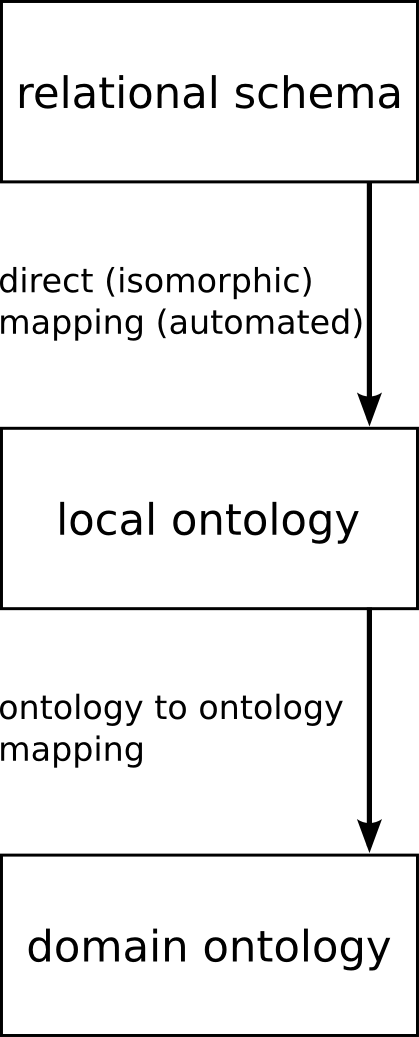
\includegraphics[width=\textwidth,height=.88\textheight,keepaspectratio]{g0}
% \end{frame}



\begin{frame}{Data Preparation}
\begin{columns}
\begin{column}{.3\textwidth}
%\color{red}\rule{\linewidth}{4pt}
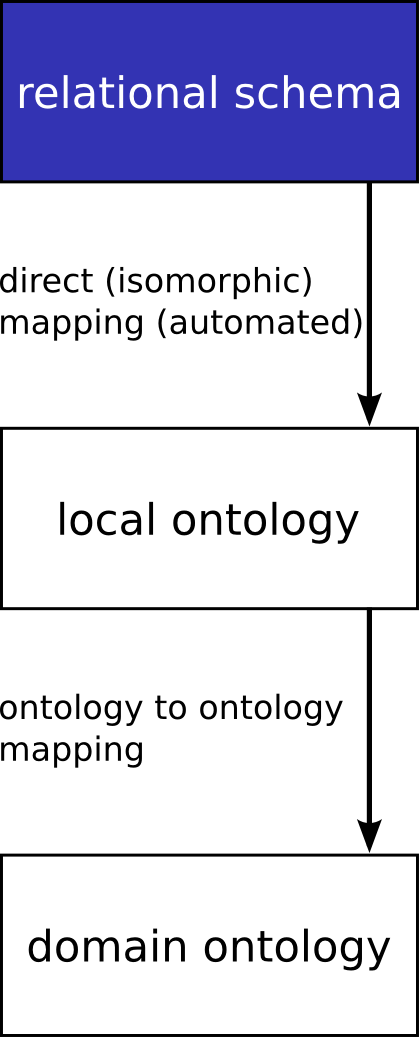
\includegraphics[width=\textwidth,height=.88\textheight,keepaspectratio]{g1}

\end{column}%
\hfill%
\begin{column}{.66\textwidth}
%\color{blue}\rule{\linewidth}{4pt}
  \centering

\begin{tabular}{lll}
  \topline
  \headcol patient\_id & birth\_date & gender \\
  \midline
  patient\_1 & 12-AUG-1956 & M \\
  \ldots & \ldots & \ldots \\
  \bottomlinec
\end{tabular}
  % \begin{tabular}{| l | l | l | l |}
  %   \hline
  %   patient\_id & birth\_date  & gender \\ \hline
  %   patient\_1  & 12-AUG-1956 & M \\
  %   \ldots  & \ldots & \ldots \\
  %   \hline
  % \end{tabular}


\adjustbox{max width=\textwidth}{
\begin{tabular}{llll}
  \topline
  \headcol medical\_case\_id  & patient\_id & admission\_date & discharge\_date \\
  \midline
    medical\_case\_100 & patient\_1  & 17-JAN-2009    & 19-JAN-2009    \\
    medical\_case\_101 & patient\_1  & 03-SEP-2009    & 27-SEP-2009    \\
    \ldots & \ldots  & \ldots    & \ldots    \\
  \bottomlinec
\end{tabular}
}
  % \adjustbox{max width=\textwidth}{
  % \begin{tabular}{| l | l | l | l|}
  %   \hline
  %   medical\_case\_id  & patient\_id & admission\_date & discharge\_date \\ \hline
  %   medical\_case\_100 & patient\_1  & 17-JAN-2009    & 19-JAN-2009    \\
  %   medical\_case\_101 & patient\_1  & 03-SEP-2009    & 27-SEP-2009    \\
  %   \ldots & \ldots  & \ldots    & \ldots    \\
  %   \hline
  % \end{tabular}}

\begin{tabular}{lll}
  \topline
  \headcol     diagnose\_id & medical\_case\_id  & ICD\_code \\
  \midline
    diagnose\_1  & medical\_case\_101 & F48      \\
    diagnose\_2  & medical\_case\_101 & T85.4    \\
    \ldots  & \ldots & \ldots   \\
  \bottomlinec
\end{tabular}
  
  % \begin{tabular}{| l | l | l |}
  %   \hline
  %   diagnose\_id & medical\_case\_id  & ICD\_code \\ \hline
  %   diagnose\_1  & medical\_case\_101 & F48      \\
  %   diagnose\_2  & medical\_case\_101 & T85.4    \\
  %   \ldots  & \ldots & \ldots   \\
  %   \hline
  % \end{tabular}

  % \begin{tabular}{| l | l | l |}
    
  % \end{tabular}
\end{column}%
\end{columns}
\end{frame}

\begin{frame}[fragile]{Data Preparation}
\begin{columns}
\begin{column}{.3\textwidth}
%\color{red}\rule{\linewidth}{4pt}
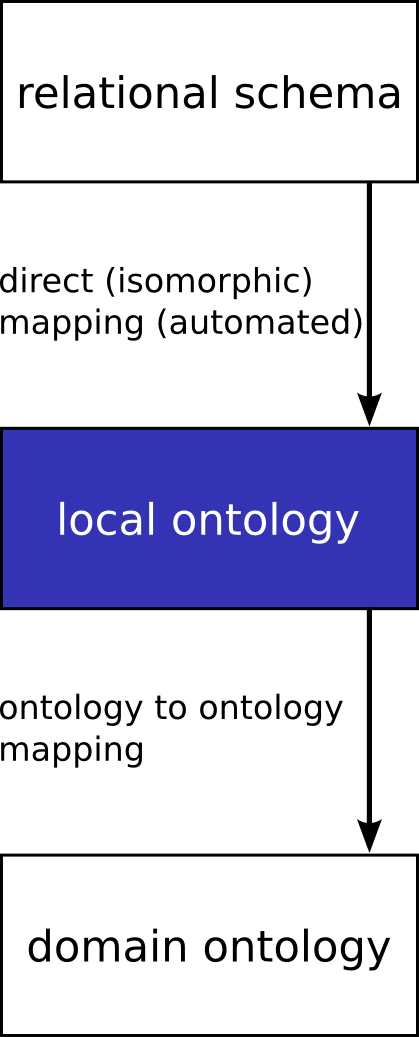
\includegraphics[width=\textwidth,height=.88\textheight,keepaspectratio]{g2}

\end{column}%
\hfill%
\begin{column}{.66\textwidth}
{\tiny
\begin{verbatim}
@prefix diagnose: <http://www.example.org/ddo/diagnose#>.
@prefix medical-case: <http://www.example.org/ddo/medical-case#>
@prefix rdfs: <http://www.w3.org/2000/01/rdf-schema#>.
@prefix xsd: <http://www.w3.org/2001/XMLSchema#>.

diagnose:Diagnose a rdfs:Class.
diagnose:diagnose-id a rdf:Property ;
                       rdfs:domain diagnose:Diagnose ;
                       rdfs:range xsd:Literal.
diagnose:medical-case-id a rdf:Property ;
                           rdfs:domain diagnose:Diagnose ;
                           rdfs:range medical-case:Medical-Case.
diagnose:icd-code a rdf:Property ;
                    rdfs:domain diagnose:Diagnose ;
                    rdfs:range xsd:Literal

...
\end{verbatim}
}
\end{column}%
\end{columns}
\end{frame}


\begin{frame}{Data Preparation}
\begin{columns}
\begin{column}{.3\textwidth}
%\color{red}\rule{\linewidth}{4pt}
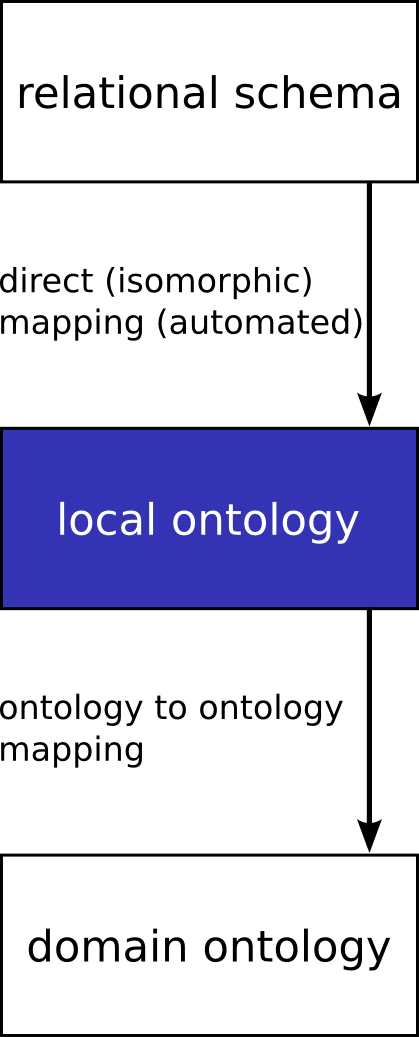
\includegraphics[width=\textwidth,height=.88\textheight,keepaspectratio]{g2}

\end{column}%
\hfill%
\begin{column}{.66\textwidth}
\begin{figure}
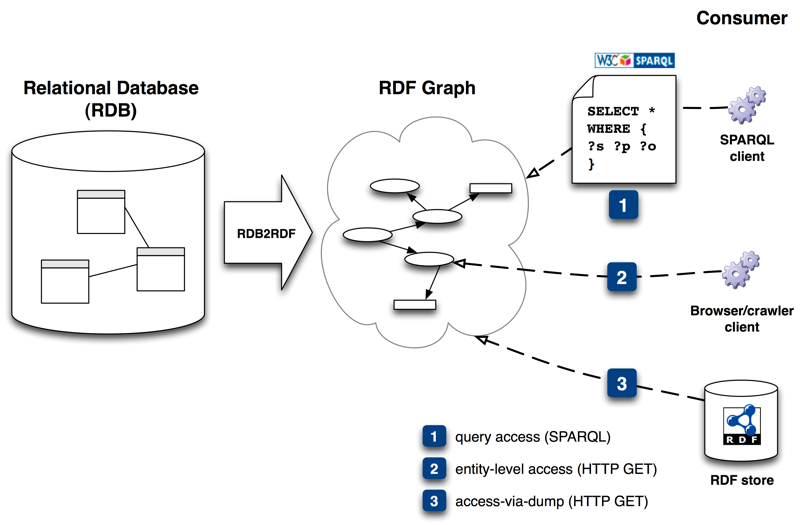
\includegraphics[width=\textwidth,height=.88\textheight,keepaspectratio]{rdb2rdf}
{\footnotesize \caption{http://www.w3.org/2001/sw/rdb2rdf/use-cases/}}
\end{figure}
\end{column}%
\end{columns}
\end{frame}


\begin{frame}[fragile]{Data Preparation}
\begin{columns}
\begin{column}{.3\textwidth}
%\color{red}\rule{\linewidth}{4pt}
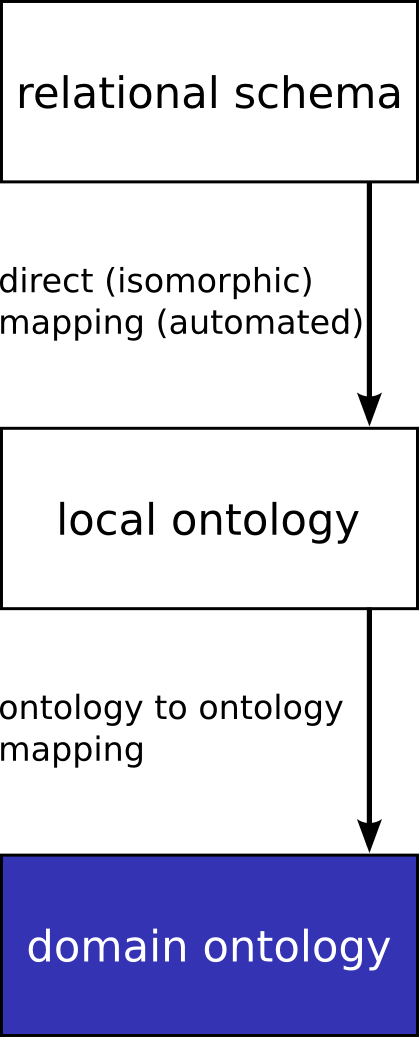
\includegraphics[width=\textwidth,height=.88\textheight,keepaspectratio]{g3}
\end{column}%
\hfill%
\begin{column}{.66\textwidth}
{\tiny
\begin{verbatim}
@prefix patient: <http://www.example.org/ddo/patient#>.
@prefix heca: <http://www.agfa.com/w3c/2009/healthCare#>.
{
    ?patient a patient:Patient.
} => {
    ?patient a heca:Patient.
}.

...
\end{verbatim}
}
\end{column}%
\end{columns}
\end{frame}






\begin{frame}[fragile]{Data Preparation}
\begin{columns}
\begin{column}{.3\textwidth}
%\color{red}\rule{\linewidth}{4pt}
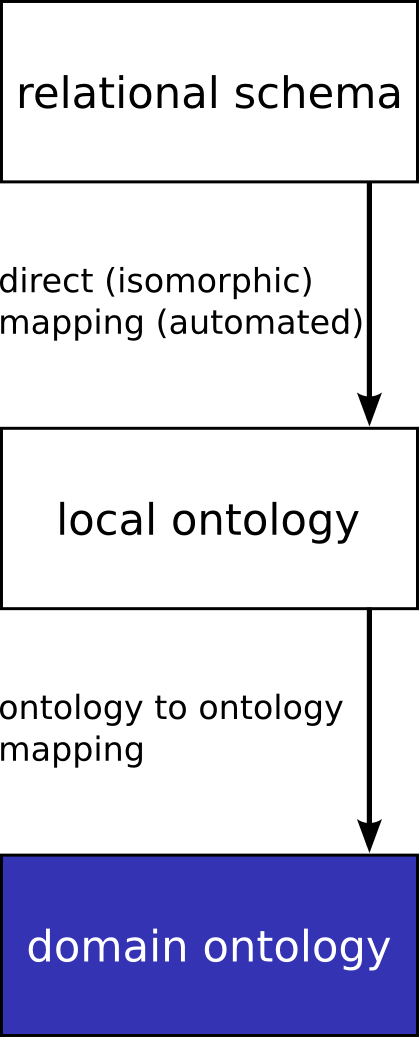
\includegraphics[width=\textwidth,height=.88\textheight,keepaspectratio]{g3}
\end{column}%
\hfill%
\begin{column}{.66\textwidth}
{\tiny
\begin{verbatim}
@prefix orgStructure: <http://www.example.org/ddo/orgStructure#>.
@prefix space: <http://eulersharp.sourceforge.net/2003/03swap/space#>.
{
    _:structure
        orgStructure:structID ?s ;
        orgStructure:innerStructID ?is .
} => {
    ?is space:containedBy ?s .
}.

{
    ?startNode space:containedBy ?middleNode .
    ?middleNode space:containedBy ?endNode .
} => {
    ?startNode space:containedBy ?endNode .
}.
\end{verbatim}
}
\end{column}%
\end{columns}
\end{frame}



\begin{frame}{Problem approach}
split problem  up AE's based on same trigger
\end{frame}

\begin{frame}{Data mining approach characteristics}
  \begin{itemize}
  \item support relational input data
  \item perform induction
  \item incorporate reverse machine learning
  \item probability
  \end{itemize}
\end{frame}

\begin{frame}{Data mining approach characteristics}
  example patient record timeline
\end{frame}


\begin{frame}{Conclusions}
  some stuff
\end{frame}


% % \begin{lstlisting}[style=rdf,float, caption={Two rules in N3, one imposes a space:containedBy relation, the other expresses the transitive closure over this relation}, label=rule_example]
% % @prefix orgStructure: <http://www.example.org/database/ddo/orgStructure#> .
% % @prefix space: <http://eulersharp.sourceforge.net/2003/03swap/space#> .

% % {
% %         _:structure 
% %                 orgStructure:structID ?s ;
% %                 orgStructure:innerStructID ?is .
% % } => {
% %         ?is space:containedBy ?s .  
% % } .

% % {
% %         ?startNode space:containedBy ?middleNode .
% %         ?middleNode space:containedBy ?endNode .
% % } => {
% %         ?startNode space:containedBy ?endNode .
% % } .
% % \end{lstlisting}

% \end{frame}
\end{document}